\chapter{Oprogramowanie i testy robota}
Oprogramowanie robota zostało napisane w języku C z użyciem dedykowanego środowiska \textit{STM32CubeIDE}. Zgodnie z dobrymi praktykami programistycznymi wykorzystano system kontroli wersji \textit{git}, a samo repozytorium znajduje się na stronie \textit{Github}. Kod jest publiczny oraz udostępniony na licencji typu open-source (GPLv3), można go znaleźć pod \href{https://github.com/trash-hold/STM32_modular_robot.git}{tym adresem}.


\section{Program główny}
Program główny składa się z kilku podstawowych segmentów, a jego uogólniony przebieg jest ziulustrowany na rysunku \ref{fig: main_program}.
    \begin{figure}[ht!]
        \centering
        \includegraphics[width=\linewidth]{rysunki/main_program/main_program_diagram.pdf}
        \caption{Kolejne etapy przebiegu programu głównego}
        \label{fig: main_program}
    \end{figure}

\paragraph*{Import plików nagłówkowych} W pierwszym etapie importowane są pliki nagłówkowe użytkownika oraz biblioteki \gls{hal}. \gls{hal} jest biblioteką opakowującą (ang. \textit{wrapper library}) funkcje operujące na rejestrach. Jej użycie pozwala na bardziej przyjazne użytkownikowi tworzenie oprogramowania dla mikrokontrolerów z rodziny STM32. Pomimo, że używanie pośredniego oprogramowania ogranicza kontrolę nad zachowaniem układu, w niniejszej pracy zdecydowano się na~jego użycie -- wynika to ze stopnia skomplikowania tworzenia własnych bibliotek najniższego stopnia abstrakcji (ang \textit{bare-metal}) oraz ilości użytych interfejsów. Oprócz HAL użyto również gotowej \href{https://www.waveshare.com/wiki/1.8inch_LCD_Module#Software}{biblioteki do obsługi wyświetlacza LCD} zapewnionej przez producenta. 

By zachować porządek oraz przejrzystość kodu, wszystkie większe funkcjonalności rozdzielono na niezależne pliki nagłówkowe. Schemat importowania plików nagłówkowych jest przedstawiony na~rysunku \ref{fig: header_include}. Dla zmniejszenia redundancji kodu i zapobiegnięciu wzajemnego importowania się plików dodano spajającą bibliotekę \texttt{system\_logic.c} oraz \texttt{system\_logic.h}, która zarządca również logiką układu

\begin{figure}[ht!]
    \centering
    \includegraphics[width=0.7\linewidth]{rysunki/main_program/header_includes.pdf}
    \caption{Schemat importowania plików nagłówkowych}
    \label{fig: header_include}
\end{figure}

\paragraph*{Deklaracja zmiennych globalnych} W kolejnym kroku deklarowane są zmienne globalne. Użyto ich głównie do deklaracji buforów, struktur związanych z pracą peryferiów oraz zmiennych definiujących pracę robota (np.: identyfikator lub rolę). Zgodnie z zasadami ''czystego kodu'' (ang. \textit{clean code)} ich ilość jest ograniczona do minimum. Było to możliwe dzięki napisaniu jak najbardziej ogólnych funkcji znajdujących się w plikach nagłówkowych.

\paragraph*{Inicjalizacja peryferiów} Następnie zachodzi inicjalizacja peryferiów, zegarów oraz innych układów potrzebnych do poprawnej pracy urządzenia. Funkcje oraz kolejność ich wykonywania są definiowanie przez środowisko programistyczne na podstawie konfiguracji wynikającej z pliku \texttt{.ioc}. W tym segmencie znajdują się również funkcje inicjalizujące urządzenia oraz ich maszyny stanów. Konfigurują one pracę akcelerometrów, serw, karty microSD, wyświetalacza LCD oraz magistrali CAN oraz odpowiadają za uruchomienie podzespołów w odpowiednich trybach. 

\paragraph*{Pętla główna} Ostatnim etapem pracy programu jest pętla główna programu, w której zarządzana jest praca peryferiów. Obsługa każdego z nich oparta jest o maszynę stanów, która z kolei jest zależna od komunikacji wewnętrznej (moduł-moduł) oraz zewnętrznej (moduł-panel sterowniczy). 

\subsection{Podstawowe struktury i typy wyliczeniowe}
W pliku \texttt{system\_logic.c} zdefiniowano kilka struktur oraz typów wyliczeniowych stanowiących podstawę do pracy robota. Pracę wszystkich układów uogólniono do wspólnej maszyny stanów opartej o typ \texttt{PERIPHERAL\_STATE}, kodów błędów typu \texttt{ReturnCode} oraz kodów komend \texttt{COM\_COMMAND}. Wszystkie stany \texttt{PERIPHERAL\_STATE} przestawione są w tabeli \ref{tab: per_state}.
    \begin{table}[ht!]
     \centering
      \begin{tabular}{ c | c | c | p{5.5cm}}
            Wartość [hex] & Nazwa stanu w kodzie & Nazwa użytkowa stanu & Opis \\ \hline \hline
            0x00 & \texttt{PER\_IDLE} & Czuwanie & Urządzenie oczekuje na nowe polecenie \\ \hline
            0x01 & \texttt{PER\_DONE} & Finalizacja & Urządzenie zakończyło wykonywanie polecenia z sukcesem \\ \hline
            0x02 & \texttt{PER\_WORKING} & Praca & Urządzenie jest w trakcie wykonywania polecenia \\ \hline
            0x03 & \texttt{PER\_WAITING} & Oczekiwanie & Urządzenie czeka na dane (używane jedynie w obsłudze magistrali CAN) \\ \hline
            0x04 & \texttt{PER\_ERROR} & Błąd & W trakcie wykonywania polecenia lub przyjmowania polecenia wystąpił błąd \\ \hline
            0x05 & \texttt{PER\_FAIL} & Awaria & Urządzenie przekroczyło limit następujących po sobie nieudanych operacji (kreślony stałą \texttt{MAX\_ERROR\_COUNT = 5})
      \end{tabular}
     \caption{\label{tab: per_state} Spis możliwych stanów urządzeń}
    \end{table}

W celu przechowywania obecnego stanu peryferium wykorzystywana jest struktura \texttt{peripheral\_state}, której definicja widoczna jest na listingu \ref{lst: per_state_struct}.
\begin{lstlisting}[language=C,
    caption={Definicja struktury peripheral\_state w pliku \texttt{system\_logic.h}},
    label={lst: per_state_struct}]
typedef struct peri_states{
	COM_COMMAND cmd;
	PERIPHERAL_STATE state;
	ReturnCode last_code;
	uint8_t error_count;
}peripheral_state;
\end{lstlisting}
W strukturze przechowywane są informację o: obecnie wykonywanej komendzie (\texttt{cmd}), obecnym stanie (\texttt{state}), ostatnim rezultacie operacji (\texttt{last\_code}) oraz liczbie błędów które nastąpiły po sobie (\texttt{error\_count}). Sama obsługa maszyny stanów ogranicza się do funkcji \texttt{PeripheralUpdateState}.
\begin{lstlisting}[language=C,
    caption={Definicja funkcji \texttt{PeripheralUpdateState}},
    label={lst: per_update_main}]
void PeripheralUpdateState(peripheral_state* per, ReturnCode status)
{
	if( status != G_SUCCESS)
	{
		if ( per->error_count >= MAX_ERROR_COUNT)
			per->state = PER_FAIL;
		else
		{
			per->error_count += 1;
			per->state = PER_ERROR;
		}
	}
	else
	{
		per->error_count = 0;
		per->state = PER_DONE;
	}

	per->last_code = status;
}
\end{lstlisting}
Funkcja widoczna na listingu \ref{lst: per_update_main} zapisuje ostatni status operacji do struktury \texttt{peripheral\_state}. W przypadku wystąpienia niepowodzenia inkrementowany jest licznik błędów, a urządzenie jest wprowadzane na jego podstawie w stan błędu lub awarii. W przeciwnym wypadku licznik błędów jest zerowany i urządzenie przechodzi w stan finalizacji. W ogólności wszystkie możliwe przejścia między stanami zilustrowane są na rysunku \ref{fig: legal_state}
    
\begin{figure}[ht!]
    \centering
    \includegraphics[width=0.55\linewidth]{rysunki/main_program/per_state_machine.pdf}
    \caption{Legalne przejścia między stanami}
    \label{fig: legal_state}
\end{figure} 

Osiągnięcie stanu awaryjnego docelowo powinno wymagać ponownego uruchomienia całego układu oraz serwisowania go. Jednak w obecnej wersji oprogramowania stany awaryjne nie są~utylizowane. Wynika to z faktu, że w trakcie debuggingu urządzenie może być celowo zmuszane do zwracania błędów w trakcie testów i jego resetowanie byłoby czasochłonne.

Jeśli chodzi o kody błędów (typu \texttt{ReturnCode}) przyjmują one wartości 8-bitowe co daje przestrzeń na 255 kodów  (plus jeden kod zarezerwowany dla poprawnych operacji). Znaczna większość funkcji znajdujących się w plikach nagłówkowych zwraca błędy. Kody są na tyle zróżnicowane by w przypadku wystąpienia problemu dało się określić dokładny obszar oprogramowania z którego pochodzi. W~przyszłości obsługa błędów może być rozbudowana i rozszerzona o przypisywanie im wag. Wybrane błędy wraz z ich opisami widoczne są w tabeli \ref{tab: error_table}.
    \begin{table}[!ht]
        \centering
        \begin{tabular}{l| c | p{6cm}}
            Nazwa błędu w kodzie & Wartość hex & Opis \\ \hline \hline 
            G\_ERROR          & 0x00 & Ogólny kod błędu \\ \hline
            G\_SUCCESS        & 0x01 & Kod sukcesu \\ \hline
            C\_MOUNT\_ERROR   & 0x02 & Nie udało się poprawnie zaincjalizować FATFS \\ \hline
            G\_FILE\_WRITE    & 0x03 & Nie udało się dokonać zapisu na kartę microSD\\ \hline
            G\_FILE\_READ     & 0x04 & Nie udało się otworzyć pliku na karcie microSD\\ \hline
            G\_COM\_OVERFLOW  & 0x05 & Przekazano ilość danych przekraczającą długość buferu magistrali CAN/UART \\ \hline
            G\_COM\_TRANSMIT  & 0x06 & Nie udało się wysłać wiadomości po magistrali CAN/UART \\ \hline
            G\_COM\_RECEIVE   & 0x07  & Nie udało się otrzymać poprawnej wiadomości z magistrali CAN/UART \\ \hline
            C\_RTC\_ERROR     & 0x08 & Błąd komunikacji z RTC \\ \hline
            C\_UART\_TRANSMIT & 0x09 & Błąd komunikacji na magistrali UART serwomechanizmu \\ \hline 
        \end{tabular}
        \caption{Pierwsze dziesięć kodów błędów}
        \label{tab: error_table}
    \end{table}

Ostatnim istotnym fragmentem logiki stojącej za obsługą maszyny stanów są kody operacji. Pozwalają one na jednoznaczne ustalenie rozkazu, które ma wykonać peryferium oraz bezpośrednio wskazują na rodzaj urządzenia, które ma go wykonać. Spis wszystkich obsługiwanych komend znajduje się w tabeli \ref{tab: per_cnd}.

\clearpage

    \begin{table}[ht!]
     \centering
      \begin{tabular}{ c | c | c | p{5.5cm}}
            Wartość [hex] & Nazwa operacji w kodzie & Peryferium & Opis \\ \hline \hline
            0x00 & \texttt{COM\_IDLE} & Wszystkie & Brak rozkazu \\ \hline
            0x01 & \texttt{COM\_SERVO\_POS\_READ} & Serwomechanizm & Odczytaj pozycje enkodera serwomechanizmu \\ \hline
            0x02 & \texttt{COM\_SERVO\_POS\_SET} & Serwomechanizm & Ustaw docelową pozycję serwomechanizmu \\ \hline
            0x03 & \texttt{COM\_SERVO\_READ\_TEMP} & Serwomechanizm & Odczyt temperatury wewnątrz obudowy serwomechanizmu \\ \hline
            0x04 & \texttt{COM\_SERVO\_PING} & Serwomechanizm & Sprawdź status serwomechanizmu \\ \hline
            0x05 & \texttt{COM\_ACC\_ANGLES\_READ} & Akcelerometr & Odczytaj zmierzone kąty nachylenia \\ \hline
            0x06 & \texttt{COM\_ACC\_PING} & Akcelerometr & Odczytaj ostatni status akcelerometru  \\
      \end{tabular}
     \caption{\label{tab: per_cnd} Spis dostępnych komend}
    \end{table}

\section{Podstawy komunikacji z modułami}
W przyszłości projektu możliwa będzie implementacja prawdziwej autonomii modułów, zarządzających swoim ruchem niezależnie od reszty układu. Wówczas komunikacja między modułowa sprowadzałaby się w znacznej większości do wymiany informacji o stanach wewnętrznych segmentów. Ze względu na zaawansowanie zagadnienia takiego sterowania nie jest ono elementem tej pracy. Zrealizowano jednak system komunikacji, który w przyszłości może zostać rozbudowany do takiej formy docelowej. W obecnej odsłonie w robocie znajduje się jeden moduł pełniący rolę kontrolera -- w efekcie odpowiada on za koordynowanie ruchem na magistrali CAN oraz UART. Pozostałe moduły pełnią rolę podrzędną wykonując rozkazy odczytywane po magistrali CAN. 
\subsection{Wiadomości w komunikacji UART}
Komunikacja moduł-panel sterowniczy została realizowana za pomocą protokołu UART, a~w~wymianie danych panel sterowniczy pełni rolę nadrzędną. Wybór tego sposobu komunikacji był uwarunkowany dwoma głównymi czynnikami. Pierwszym z nich jest prostota tego rodzaju transmisji, oprócz bitów stopu, startu oraz opcjonalnego bitu parzystości ramka zawiera jedynie dane. Oznacza to, że konfiguracja, uruchomienie oraz obsługa interfejsu jest prostsza w stosunku do SPI czy I$^2$C. Drugim powodem jest powszechność interfejsu UART. Jest on obecny w większości mikrokontrolerów, a ponadto można nabyć przejściówki USB-UART, które umożliwią transmisję również z poziomu komputera personalnego przy niewielkim nakładzie finansowym. Daje to pole to przyszłej rozbudowy systemu -- obecna komunikacja przewodowa może zostać łatwo zamieniona w bezprzewodową dodając na pokładzie robota odbiornik-nadajnik, który powtarzałby wiadomości przesłane po Wifi, BLE czy jakimkolwiek innym protokołem bezprzewodowym. 

Jednocześnie trzeba mieć na uwadze, że ta metoda transmisji nie jest idealna. Pierwszym problemem jest asynchroniczność protokołu, powodująca możliwe błędne odczytywanie danych przy długich transmisjach w wyniku różnic próbkowania sygnału. Drugim znacznym minusem jest brak informacji zwrotnej o otrzymaniu wiadomości przez urządzenia na magistrali. 

Mając na uwadze powyższe zdefiniowano dwa podstawowe formaty budowy wiadomości transmisji UART -- ramkę rozkazu oraz ramkę odpowiedzi. Ta druga ma na celu zmitygowanie problemu, którym jest brak potwierdzenia przyjęcia transmisji -- niezależnie od poprawności danych przychodzących do modułu, panel sterowniczy powinien otrzymać odpowiedź. Przykładowa wymiana między urządzeniami jest widoczna na ilustracji \ref{fig: gen_uart_frame}.

    \begin{figure}[ht!]
        \centering
        \includegraphics[width=0.6\linewidth]{rysunki/basic_com/uart_tx_rx.pdf}
        \caption{Generalny schemat wymiany wiadomości}
        \label{fig: gen_uart_frame}
    \end{figure} 

 Maksymalny czas między ostatnim bajtem rozkazu i pierwszym bajtem odpowiedzi wynosi 5s i jest zdefiniowany w logice panelu sterowniczego.

    \begin{dframe}[ht!]
        \centering
        \begin{bytefield}[endianness=little, bitwidth = 0.19\linewidth, bitheight = 30pt, boxformatting = {\centering \small}]{5}
            \bitbox{1}{Ilość bajtów = N} & \bitbox{1}{ID modułu} & \bitbox{1}{Kod operacji}
            & \bitbox{1}{$\hdots$} & \bitbox{1}{Suma kontrolna} \\
        \end{bytefield}
        \caption{\label{tab: transmit_frames} Ogólna ramka rozkazu}
    \end{dframe}

 Budowa ramki rozkazu jest widoczna na schemacie \ref{tab: transmit_frames}. Wiadomość rozpoczyna się od pojedynczego bajtu informującego o liczbie wszystkich danych, które powinny zostać otrzymane w ramach tej wiadomości. Następnie nadawany jest 8-bitowy identyfikator modułu, do którego powinien dotrzeć rozkaz. Później transmitowany jest kod operacji. Kolejne bajty zależne są od rodzaju wydawanego rozkazu. Całość kończona jest sumą kontrolną (ang. \textit{checksum}), która jest negacją sumy wszystkich poprzedzającej ją bajtów. Najdłuższe poprawne transmisje liczą 10 ramek UART oznacza to, że problem dotyczący ''gubienia'' danych nie powinien zachodzić. Jednak gdyby nastąpił, przed przyjęciem niepoprawnych danych chroni dodane pole sumy kontrolnej. W obecnej wersji istnieją dwa formaty rozkazów widoczne na schematach \ref{frame: servo_set_pos_trans} oraz \ref{frame: transmit_frames_all}.

 \clearpage

    \begin{dframe}[ht!]
        \centering
        \textbf{Ramka rozkazu \texttt{SERVO\_SET\_POS}} \\[9pt]
        \begin{bytefield}[endianness=little, bitwidth = 0.095\linewidth, bitheight = 60pt, boxformatting ={\centering \small}]{10}
            \bitheader{0-9} \\
            \bitbox{1}{0x0A} & \bitbox{1}{ID modułu} & \bitbox{1}{Kod operacji}
            & \bitbox{1}{ID serwa} & \bitbox{1}{Przyśpie -szenie} & \bitbox{1}{LB pozycji} & \bitbox{1}{HB pozycji} & \bitbox{1}{LB prędkości} & \bitbox{1}{HB prędkości} \bitbox{1}{Suma kontrolna} \\
        \end{bytefield} \\[7pt]
        \caption{\label{frame: servo_set_pos_trans} Ramka rozkazu \texttt{SERVO\_SET\_POS}}
    \end{dframe}

    \begin{dframe}[!ht]
        \centering
        \textbf{Ramka reszty rozkazów}\\[9pt]
        \begin{bytefield}[endianness=little, bitwidth = 0.19\linewidth, bitheight = 30pt, boxformatting ={\centering \small}]{5}
            \bitheader{0-4} \\
            \bitbox{1}{0x05} & \bitbox{1}{ID modułu} & \bitbox{1}{Kod operacji}
            & \bitbox{1}{ID peryferium} & \bitbox{1}{Suma kontrolna} \\
        \end{bytefield}
        \caption{\label{frame: transmit_frames_all} Ramka reszty rozkazów}
    \end{dframe}

Ramka wiadomości ma analogiczną strukturę i jest widoczna na schemacie \ref{frame: message_uart_frame}. W jej przypadku pole komendy operacji zostało zamienione na pole statusu. Jest tak dlatego, że kod operacji jest zbędny do zidentyfikowania ramki rozkazu, na którą odpowiadają przychodzące dane. Wynika to z konstrukcji panelu, który zakłada wydawanie instrukcji pojedynczo. By umożliwić wymianę wielu transmisji w jednym momencie należało by na przykład rozszerzyć obie ramki o unikalny identyfikator.

    \begin{dframe}[ht!]
        \centering
        \begin{bytefield}[endianness=little, bitwidth = 0.19\linewidth, bitheight = 30pt, boxformatting = {\centering \small}]{5}
            \bitbox{1}{Ilość bajtów = N} & \bitbox{1}{ID modułu} & \bitbox{1}{Status operacji}
            & \bitbox{1}{$\hdots$} & \bitbox{1}{Suma kontrolna} \\
        \end{bytefield}
        \caption{\label{frame: message_uart_frame} Ogólna ramka wiadomości}
    \end{dframe}

Obecnie występują cztery formaty ramek wiadomości, są one widoczne na schematach: \ref{frame: servo_pos_msg}, \ref{frame: status_msg}, \ref{frame: ans_acc_angles} oraz \ref{frame: ans_gen}.

    \begin{dframe}[ht!]
        \centering
        \begin{bytefield}[endianness=little, bitwidth = 0.159\linewidth, bitheight = 60pt, boxformatting ={\centering \small}]{6}
            \bitheader{0-5} \\
            \bitbox{1}{0x06} & \bitbox{1}{ID modułu} & \bitbox{1}{0x01}
            & \bitbox{1}{Górny bajt pozycji} & \bitbox{1}{Dolny bajt pozycji} & \bitbox{1}{Suma kontrolna}
        \end{bytefield} 
        \caption{\label{frame: servo_pos_msg} Ramka odpowiedzi dla \texttt{SERVO\_READ\_POS}}
        \vspace{12pt}
        \begin{bytefield}[endianness=little, bitwidth = 0.2375\linewidth, bitheight = 30pt, boxformatting ={\centering \small}]{4}
            \bitheader{0-3} \\
            \bitbox{1}{0x04} & \bitbox{1}{ID modułu} & \bitbox{1}{Status} & \bitbox{1}{Suma kontrolna} \\
        \end{bytefield}
        \caption{\label{frame: status_msg} Ramka statusowa}
    \end{dframe}

    \clearpage   
    \begin{dframe}[ht!]
        \centering
        \begin{bytefield}[endianness=little, bitwidth = 0.095\linewidth, bitheight = 60pt, boxformatting ={\centering \small}]{10}
            \bitheader{0-9} \\
            \bitbox{1}{0x0A} & \bitbox{1}{ID modułu} & \bitbox{1}{0x01}
            & \bitbox{1}{Część całości kąta A} & \bitbox{1}{Część ułamkowa kąta A} & \bitbox{1}{Część całości kąta B} & \bitbox{1}{Część ułamkowa kąta B} & \bitbox{1}{Część całości kąta C} & \bitbox{1}{Część ułamkowa kąta C} \bitbox{1}{Suma kontrolna}
        \end{bytefield}
        \caption{\label{frame: ans_acc_angles} Ramka odpowiedzi dla \texttt{ACC\_ANGLES\_READ}}
        \vspace{12pt}
        \begin{bytefield}[endianness=little, bitwidth = 0.19\linewidth, bitheight = 30pt, boxformatting ={\centering \small}]{5}
            \bitheader{0-3} \\
            \bitbox{1}{0x05} & \bitbox{1}{ID modułu} & \bitbox{1}{Status} & \bitbox{1}{ID peryferium} & \bitbox{1}{Suma kontrolna} \\
        \end{bytefield}
        \caption{\label{frame: ans_gen} Ramka odczytu pozostałych danych}
    \end{dframe}

%\subsection{Wiadomości w komunikacji CAN}
%Komunikacja moduł-moduł jest realizowana z użyciem protokołu CAN, którego dokładne działanie omówiono w rozdziale drugim.
\section{Obsługa serwomechanizmu}
W strukturze serwa zintegrowane są enkoder absolutny oraz czujnik temperatury. Pozwalają one na zbieranie podstawowych informacji o pracy serwa. Wszelka komunikacja z urządzeniem jest możliwa przez UART w wydaniu jednoprzewodowym -- oznacza to, że transmisja i odbiór ramek odbywa się w trybie pół-dupleksu (ang. \textit{half-duplex}). Mikrokontroler pełni rolę nadrzędną natomiast serwomechanizm podrzędną. Kod obsługujący pracę serwomechanizmu jest umieszczony w plikach \texttt{ST3020.h} oraz \texttt{ST3020.c}.

Znacznymi problemami w opracowaniu obsługi serwa były: brak dokumentacji technicznej, opisu pracy urządzenia czy instrukcji użytkowania. Najbardziej wartościowym źródłem informacji były \href{https://www.waveshare.com/wiki/ST3020_Servo#Software}{biblioteka oraz aplikacja} przeznaczone na mikrokontrolery z rodziny AVR (Arduino lub ESP32). Na ich podstawie udało się w częściowo zdefiniować zasady działania serwa. Zadawanie oraz odczytywanie parametrów pracy odbywa się za pomocą operacji zapisu lub odczytu komórek pamięci SRAM lub EPROM. W pamięci trwałej serwomechanizm przechowuje przede wszystkim swój identyfikator, kod producenta oraz szybkość transmisji. W pamięci ulotnej znajdują się natomiast obecne parametry urządzenia takie jak zadany kąt, obecny kąt, temperatura, odczyt napięcia oraz prądu. W tabeli \ref{tab: servo_memory_map} pokazano mapę pamięci urządzenia.
\begin{center}
    \begin{longtable}[c]{|l|c|}
        \hline
        \multicolumn{2}{|c|}{\textbf{EPROM (Wyłącznie odczyt)}} \\
        \hline
        \textbf{Nazwa rejestru} & \textbf{Adres rejestru [dec]} \\
        \hline
        \endfirsthead
        \hline
        \multicolumn{2}{|c|}{\textbf{EPROM (Odczyt i zapis)}} \\
        \hline
        \textbf{Nazwa rejestru} & \textbf{Adres rejestru [dec]} \\
        \hline
        \endhead
        \hline
        \multicolumn{2}{|c|}{\textbf{SRAM (Odczyt i zapis)}} \\
        \hline
        \textbf{Nazwa rejestru} & \textbf{Adres rejestru [dec]} \\
        \hline
        \endhead
        \hline
        \caption{\label{tab: servo_memory_map} Mapa pamięci serwa}
        \endfoot
        
        \hline
        SCSCL\_VERSION\_L & 3 \\
        \hline
        SCSCL\_VERSION\_H & 4 \\
        \hline
        
        \multicolumn{2}{|c|}{\textbf{EPROM (Odczyt i zapis)}} \\
        \hline
        \textbf{Nazwa rejestru} & \textbf{Adres rejestru [dec]} \\
        \hline
        SCSCL\_ID & 5 \\
        \hline
        SCSCL\_BAUD\_RATE & 6 \\
        \hline
        SCSCL\_MIN\_ANGLE\_LIMIT\_L & 9 \\
        \hline
        SCSCL\_MIN\_ANGLE\_LIMIT\_H & 10 \\
        \hline
        SCSCL\_MAX\_ANGLE\_LIMIT\_L & 11 \\
        \hline
        SCSCL\_MAX\_ANGLE\_LIMIT\_H & 12 \\
        \hline
        SCSCL\_CW\_DEAD & 26 \\
        \hline
        SCSCL\_CCW\_DEAD & 27 \\
        \hline

        SCSCL\_TORQUE\_ENABLE & 40 \\
        \hline
        SCSCL\_GOAL\_POSITION\_L & 42 \\
        \hline
        SCSCL\_GOAL\_POSITION\_H & 43 \\
        \hline
        SCSCL\_GOAL\_TIME\_L & 44 \\
        \hline
        SCSCL\_GOAL\_TIME\_H & 45 \\
        \hline
        SCSCL\_GOAL\_SPEED\_L & 46 \\
        \hline
        SCSCL\_GOAL\_SPEED\_H & 47 \\
        \hline
        SCSCL\_LOCK & 48 \\
        \hline
        SCSCL\_PRESENT\_POSITION\_L & 56 \\
        \hline
        SCSCL\_PRESENT\_POSITION\_H & 57 \\
        \hline
        SCSCL\_PRESENT\_SPEED\_L & 58 \\
        \hline
        SCSCL\_PRESENT\_SPEED\_H & 59 \\
        \hline
        SCSCL\_PRESENT\_LOAD\_L & 60 \\
        \hline
        SCSCL\_PRESENT\_LOAD\_H & 61 \\
        \hline
        SCSCL\_PRESENT\_VOLTAGE & 62 \\
        \hline
        SCSCL\_PRESENT\_TEMPERATURE & 63 \\
        \hline
        SCSCL\_MOVING & 66 \\
        \hline
        SCSCL\_PRESENT\_CURRENT\_L & 69 \\
        \hline
        SCSCL\_PRESENT\_CURRENT\_H & 70 \\
        \hline
    \end{longtable}
    
\end{center}
    
\subsection{Zapis do pamięci serwa}
Transmisja zapisu ma minimalną długość 6 ramek i składa się zawsze z dwóch transmisji, roboczo nazywanymi nagłówkiem oraz wiadomością właściwą. Ogólny format wiadomości widoczny jest na~schemacie \ref{frame: servo_transmit_frames}.
\begin{dframe}[!ht]
    \centering
    \newcommand{\bitlabel}[2]{%
            \bitbox[]{#1}{%
            \raisebox{0pt}[4ex][0pt]{%
            {\fontsize{10}{7}\selectfont#2}%
            }%
        }%
    }

    \begin{bytefield}[endianness=little, bitwidth = 0.125\linewidth, bitheight = 60pt, boxformatting = {\centering \small}]{8}
        \bitlabel{2}{Bajty synchronizujące} & \bitlabel{4}{Nagłówek} & \bitlabel{2}{Wiadomość właściwa} \\
        \bitbox{1}[bgcolor = lightgray]{0xFF} & \bitbox{1}[bgcolor = lightgray]{0xFF} & \bitbox{1}{ID serwa} & \bitbox{1}{Długość tranmisji = N+3}  & \bitbox{1}{Komenda} & \bitbox{1}{Adres pamięci serwa} & \bitbox{1}{N danych} & \bitbox{1}{Suma kontrolna} \\
    \end{bytefield}
    \caption{\label{frame: servo_transmit_frames} Ogólna struktura wiadomości serwomechanizmu}
\end{dframe} 

 Pierwsza wiadomość musi zaczynać się od dwóch bajtów synchronizujących (o wartości 0xFF). Pozwalają one na jednoznaczne zidentyfikowanie początku wiadomości przez odbiorniki. Nie są one liczone jako faktyczna treść wymiany informacji -- wyklucza je się z określania długości transmisji oraz sumy kontrolnej. Następnie podawany jest identyfikator serwa, który porównywany będzie z komórką pamięci EPROM (\texttt{SCSCL\_ID}). Kolejny bajt mówi o długości transmisji równej N + 3, gdzie N to ilość wysyłanych bajtów danych do pamięci. Koniec treści nagłówka stanowią bajty kodu operacji (zgodnego z logiką serwa) oraz adresu pierwszego rejestru danych. Transmisja wiadomości właściwej składa się z N bajtów danych, które powinny zostać umieszczone w kolejnych komórkach pamięci serwomechanizmu. Koniec całej wymiany stanowi suma kontrolna będąca negacją sumy wszystkich bajtów obu transmisji.

 Serwomechanizm przyjmuje trzy rodzaje komend:
    \begin{itemize}
        \item Zapis do pamięci = 0x03,
        \item Odczyt pamięci = 0x02,
        \item Ping = 0x01
    \end{itemize}
Należy dodać, że w przypadku komedy ping występuje odstępstwo od formatu \ref{frame: servo_transmit_frames}, bajt adresu pamięci serwa jest wówczas pomijany.

Funkcją odpowiadającą za transmisję wiadomości jest \texttt{ServoWrite}, której deklaracja przedstawiona jest w listingu \ref{lst: def_servowrite}.
\begin{lstlisting}[language=C,
caption={Deklaracja funkcji \texttt{ServoWrite}},
label={lst: def_servowrite}]
    static ReturnCode ServoWrite(UART_HandleTypeDef* uart, uint8_t cmd, uint8_t reg, uint8_t *data_buffer, uint8_t len)
\end{lstlisting}
Zasięg funkcji ogranicza się do pliku \texttt{ST3020\_servo.c}, natomiast przyjmowane parametry to kolejno: wskaźnik do struktury interfejsu UART bilbioteki HAL, kod operacji, pierwszy adres rejestru, do~którego ma nastąpić zapis danych, wskaźnik do buforu zawierającego dane do transmisji, liczba danych w buforze.
\begin{lstlisting}[language=C,
caption={Początek funkcji \texttt{ServoWrite}},
label={lst: servowrite_transmiten}]
    HAL_StatusTypeDef status = HAL_HalfDuplex_EnableTransmitter(uart);
    if (status != HAL_OK)
    {
        return C_UART_TRANSMIT;
    }
    
    const uint8_t buffer_size = (len > 5) ? len + 1 : 6;
    uint8_t tx_buffer[buffer_size];
\end{lstlisting}
Jak widoczne w listingu \ref{lst: servowrite_transmiten}, w pierwszej kolejności następuje zmiana roli pełnionej przez mikrokontroler na magistrali -- wymuszane jest by stał się transmiterem. Jest to realizowane za pomocą funkcji \texttt{HAL\_HalfDuplex\_EnableTransmitter}. Następnie obliczana jest potrzebna wielkość bufora danych i jest on inicjalizowany.
\begin{lstlisting}[language=C,
caption={Fragment \texttt{ServoWrite} odpowiadający za uzupełnienie treści nagłówka},
label={lst: servowrite_header}]
    tx_buffer[0] = 0xFF;
    tx_buffer[1] = 0xFF;
    tx_buffer[2] = 0x01;		
    tx_buffer[3] = len + 0x03;	
    tx_buffer[4] = cmd;		    
    tx_buffer[5] = reg;			
\end{lstlisting}
W kolejnym kroku zapisywane są kolejne bajty nagłówka \ref{lst: servowrite_header} zgodne z wcześniej przedstawionym formatem \ref{frame: servo_transmit_frames}.

\begin{lstlisting}[language=C,
caption={Fragment \texttt{ServoWrite} odpowiadający za transmisję nagłówka},
label={lst: servowrite_transmitheader}]
    uint8_t checksum = 0;
    for (uint8_t i = 0; i < len; i++)
    {
        checksum += *(data_buffer + i);
    }
    
    for ( uint8_t i = 2; i < 6; i++)
    {
        checksum += tx_buffer[i];
    }
    
    status = HAL_UART_Transmit(uart, tx_buffer, 6, SERVO_TIMEOUT);
    if (status != HAL_OK)
        return C_UART_TRANSMIT;
\end{lstlisting}
 Przed wysłaniem nagłówka liczona jest suma kontrolna. Jest to realizowane poprzez dwie pętle \texttt{for} iterujące kolejne indeksy buforu nagłówka oraz treści właściwej, a następnie dodając ich zawartość do zmiennej \texttt{checksum}. By nie powodować niepotrzebnych opóźnień między transmisjami nagłówka a wiadomości właściwej suma kontrolna jest liczona przed rozpoczęciem pierwszej transmisji. W~ostatnim kroku przeprowadza się pierwszą z dwóch transmisji, które realizowane są z użyciem funkcji \texttt{HAL\_UART\_Transmit}. Pełna implementacja tego etapu jest widoczna w listingu \ref{lst: servowrite_transmitheader}.

\begin{lstlisting}[language=C,
    caption={Fragment \texttt{ServoWrite} odpowiadający za transmisję wiadomości właściwej},
    label={lst: servowrite_transmitmsg}]
    for (uint8_t i = 0; i < len; i++)
    {
        tx_buffer[i] = *(data_buffer + i);
    }
    tx_buffer[len] = (~checksum);
    
    status = HAL_UART_Transmit(uart, tx_buffer, len + 1, SERVO_TIMEOUT);
    if( status != HAL_OK)
        return C_UART_TRANSMIT;
    
    return G_SUCCESS;
\end{lstlisting}
Jak widoczne w listingu \ref{lst: servowrite_transmitmsg}, dane z buforu przepisywane są do buforu pomocniczego, a na jego końcu dodaje się pole stanowiące negację obliczonej sumy kontrolnej. Po tych operacjach otrzymuje się treść wiadomości właściwej. Jeśli w trakcie transmisji nie wystąpią błędy, całość funkcji zwraca kod sukcesu.

\subsection{Odczyt pamięci serwa}
Do odczytywania zawartości komórek pamięci serwa służy funkcja \texttt{ServoRead}, której deklaracja jest widoczna na listingu \ref{lst: servoread_dec}.
\begin{lstlisting}[language=C,
caption={Deklaracja funkcji \texttt{ServoRead}},
label={lst: servoread_dec}]
    ReturnCode ServoRead(uint8_t servo_line, uint8_t reg, uint8_t* data_buffer, uint8_t bytes);
\end{lstlisting}
Przyjmowane parametry to kolejno: indeks linii serwa definiujący magistralę UART, adres rejestru pierwszej komórki pamięci serwa do odczytu, wskaźnik do buforu w którym zapisane będą pobrane bajty, ilość bajtów do odczytu. Funkcja jest dostępna z poziomu programu głównego.
\begin{lstlisting}[language=C,
caption={Początek funkcji \texttt{ServoRead}},
label={lst: servoread_handle}]
    UART_HandleTypeDef* uart;
        switch(servo_line)
        {
            case 0x00:
                uart = uart_s1;
                break;
            case 0x01:
                uart = uart_s2;
                break;
            default:
                return C_UART_HANDLE;
        }
\end{lstlisting}
Proces zapisu zaczyna się od pobrania odpowiedniego wskaźnika na strukturę \texttt{UART\_HandleTypeDef}, która jest kluczowa dla obsługi magistrali przez bibliotekę HAL. Interfejs jest wybierany w zależności od pobranego indeksu linii serwa, co jest widoczne w listingu \ref{lst: servoread_handle}.
\begin{lstlisting}[language=C,
caption={Transmisja zażądająca odczytu danych},
label={lst: servoread_header}]
    if (ServoWrite(uart, SERVO_READ_INS, reg, &bytes, 1) != G_SUCCESS)
        return G_SERVO_WRTIE;
\end{lstlisting}
W pierwszej kolejności wysyłana jest wiadomość zażądająca N bajtów danych. Transmisja jest wykonywana przez wcześniej przygotowaną funkcję lokalną, która była opisana w poprzedniej sekcji. Jak widoczne w listingu \ref{lst: servoread_header} jest to operacja znacznie uproszczona dzięki zbudowanemu interfejsowi.
\begin{lstlisting}[language=C,
    caption={Odczyt wiadomości zawierającej dane pobierane z pamięci serwa},
    label={lst: servo_read}]
    HAL_StatusTypeDef status = HAL_HalfDuplex_EnableReceiver(uart);
	if (status != HAL_OK)
		return C_UART_RECEIVE;

	uint8_t header_buffer[5];
	HAL_UART_Receive(uart, header_buffer, 1, SERVO_TIMEOUT);
	if( header_buffer[0] != 0xFF)
		HAL_UART_Receive(uart, header_buffer, 5, SERVO_TIMEOUT);
	else
		HAL_UART_Receive(uart, header_buffer + 1, 4, SERVO_TIMEOUT);

	status = HAL_UART_Receive(uart, data_buffer, bytes, SERVO_TIMEOUT);
	if (status != HAL_OK)
		return C_UART_RECEIVE
        
    if ( (header_buffer[2] != 0x01) || (header_buffer[3] != bytes + 0x02) )
            return C_UART_RECEIVE;
    return G_SUCCESS;
\end{lstlisting}
Listing \ref{lst: servo_read} przedstawia proces odbioru wiadomości od serwomechanizmu. Najpierw magistrala mikrokontrolera jest ustawiana w tryb odbiornika z użyciem funkcji \texttt{HAL\_HalfDuplex\_EnableReceiver} bilioteki HAL. W kolejnym kroku odczytywana jest pierwszy bajt transmisji i sprawdzane jest czy jest równy $0xFF$. Jeśli nie odebrane dane są odrzucane. Podczas pracy z serwomechanizem nie zdarzyło się, by wymagane było dłuższe oczekiwanie na poprawne odebranie bajtów synchronizująch niż pojedyncza transmisja, dlatego nie ma potrzeby nasłuchiwania wiadomości więcej niż raz. Finalnie otrzymuje się 5 bajtów stanowiących nagłówek odczytywanej wiadomości. Następnie magistrala jest ponownie nasłuchiwana i odczytywane są bajty wiadomości właściwej. Na koniec weryfikowana jest zawartość nagłówka. Jeśli bajty długości transmisji oraz identyfikator serwomechanizmu są zgodne, zwracany jest kod sukcesu. 

\subsection{Polecenie ping serwomechanizmu}
Ostatnią funkcją bezpośrednio obsługującą magistrale UART jest \texttt{ServoPing}. Służy ona do~weryfikacji poprawności połączenia z serwomechanizmem. Deklaracja funkcji jest widoczna w~listingu~\ref{lst: servoping_dec}.
\begin{lstlisting}[language=C,
    caption={Deklaracja funkcji realizującej operację ping},
    label={lst: servoping_dec}]
    ReturnCode ServoPing(uint8_t servo_line, uint8_t id);
\end{lstlisting}
Przyjmowane są dwa argumenty: indeks magistrali serwa oraz identyfikator serwa. Funkcja dostępna jest z poziomu programu głównego.
\begin{lstlisting}[language=C,
    caption={Wiadomość zażądająca od serwomechanizmu operację ping},
    label={lst: ping_transmit}]
    HAL_StatusTypeDef status = HAL_HalfDuplex_EnableTransmitter(uart);
	if (status != HAL_OK)
	{
		return C_UART_TRANSMIT;
	}

	uint8_t buffer[6];
	uint8_t checksum = ~(id + 0x02 + 0x01);
	buffer[0] = 0xFF;
	buffer[1] = 0xFF;
	buffer[2] = id;	
	buffer[3] = 0x02;
	buffer[4] = 0x01;

	status = HAL_UART_Transmit(uart, buffer, 5, SERVO_TIMEOUT);
	if (status != HAL_OK)
		return C_UART_TRANSMIT;

	status = HAL_UART_Transmit(uart, &checksum, 1, SERVO_TIMEOUT);
		if (status != HAL_OK)
			return C_UART_TRANSMIT;
\end{lstlisting}
W pierwszej kolejności tak jak w wypadku \texttt{ServoWrite} mikrokontroler jest przełączony w tryb transmitera za pomocą funkcji \texttt{HAL\_HalfDuplex\_EnableTransmitter}. Wiadomość nagłówka różni się od zwykłej transmisji tym, że nie posiada bajtu informującego o adresie rejestru serwa co~jest widoczne w listingu \ref{lst: ping_transmit}. Reszta ramek danych pozostaje analogiczna. Widoczne jest że, treść wiadomości właściwej ogranicza się do sumy kontrolnej. Ponownie następują dwie transmisje.
\begin{lstlisting}[language=C,
    caption={Odbiór wiadomości ping},
    label={lst: ping_receive}]
    status = HAL_HalfDuplex_EnableReceiver(uart);
    if (status != HAL_OK)
        return C_UART_RECEIVE;
    
    status = HAL_UART_Receive(uart, buffer, 1, SERVO_TIMEOUT);
    if (status != HAL_OK)
        return C_UART_RECEIVE;
    
    if(buffer[0] != 0xFF)
        status = HAL_UART_Receive(uart, buffer, 6, SERVO_TIMEOUT);
    else
        status = HAL_UART_Receive(uart, buffer + 1, 5, SERVO_TIMEOUT);
    
    if (status != HAL_OK)
        return C_UART_RECEIVE;
\end{lstlisting}
Listing \ref{lst: ping_receive} przedstawia część funkcji \texttt{ServoPing} odpowiedzialnej za odbiór wiadomości od serwomechanizmu. W pierwszej kolejności urządzenie wchodzi w tryb odbiornika i przeprowadza odczyt analogiczny do tego w funkcji \texttt{ServoRead} \ref{lst: servo_read}. Jednak, ponieważ jakość transmisji jest oceniana na podstawie treści treści wiadomości właściwej ale również nagłówka, funkcja ta nie jest tu~wywoływana. Ponownie odczytywany jest pierwszy bajt, jeśli jest zgodny z oczekiwaną wartością bajtów synchronizujących odczytywane jest kolejne 5 bajtów. W przeciwnym wypadku pierwsze dane są odrzucane i nasłuchiwane jest kolejne 6 bajtów. 
\begin{lstlisting}[language=C,
    caption={Weryfikacja wiadomości ping},
    label={lst: servoping_verify}]
    if ( buffer[2] != id )
        return G_SERVO_READ;
    
    if ( buffer[3] != 0x02)
        return G_SERVO_READ;
    
    checksum = buffer[2] + buffer[3] + buffer[4];
    checksum = ~checksum;
    if ( checksum != buffer[5] )
        return G_SERVO_READ;
    
    return G_SUCCESS;
\end{lstlisting}
Ostatni etap operacji ping przedstawia listing \ref{lst: servoping_verify}. Walidowane są pola bitowe związane z~identyfikatorem serwomechanizmu, długością transmisji oraz sumą kontrolną. Jeśli nie wykryto żadnej niezgodności oraz wszystkie transmisje były przeprowadzone poprawnie, funkcja zwraca kod \texttt{G\_SUCCESS}. Jest to równoważne z dostarczeniem informacji zwrotnej o poprawnej pracy magistrali jak i samego urządzenia.

\subsection{Funkcje pomocnicze}
W celu ograniczenia redundancji kodu i uproszczeniu przepływu informacji między kolejnymi elementami programu głównego dodano kilka funkcji pomocniczych. Uporządkowują one również interfejs obsługi serwomechanizmu. 

Pierwszą z funkcji pomocniczych jest \texttt{ServoSetPos}, która jak wskazuje nazwa pozwala na zdanie pozycji serwomechanizmowi, którą powinien osiągnąć z określoną prędkością i przyśpieszeniem. Niestety producent nie zdefiniował, jak powyższe wartości są interpretowane przez sterownik układu. Na podstawie dokonanych obserwacji można przypuszczać, że podawane wartości są odpowiednio maksymalną prędkością oraz maksymalnym przyśpieszeniem. 
\begin{lstlisting}[language=C,
    caption={Deklaracja funkcji \texttt{ServoSetPos}}
    label={lst: setpos_dec}]
    ReturnCode ServoSetPos(uint8_t servo_line, int16_t pos, uint16_t speed, uint8_t acc)
\end{lstlisting}
Zgodnie z deklaracją \ref{lst: setpos_dec} funkcja przyjmuje kolejno: indeks magistrali serwa, pozycję (mogącą być liczbą niedodatnią), prędkość oraz przyśpieszenie.
\begin{lstlisting}[language=C,
caption={Fragment kodu odpowiadający za zapis nowej pozycji do pamięci serwa},
label={lst: setpos_pos}]
    if(pos < 0)
    {
        pos = -pos;
        pos |= (0x01 << 15);
    }
    
    uint8_t buff[7];
    buff[0] = acc;
    buff[1] = (uint8_t) (pos & 0x00FF);
    buff[2] = (uint8_t) ((pos & 0xFF00) >> 8);
    buff[3] = 0x00;
    buff[4] = 0x00;
    buff[5] = (uint8_t) (speed & 0x00FF);
    buff[6] = (uint8_t) ((speed & 0xFF00) >> 8);
    
    return ServoWrite(uart, SERVO_WRITE_INS, SERVO_ACC_REG, buff, 7);
\end{lstlisting}
W listingu \ref{lst: setpos_pos} przedstawiony jest odpowiedni zapis danych do transmisji oraz przekazanie wiadomości na magistralę. Kodowanie liczb niedodatnich jest inna niż w przypadku klasycznej zmiennej typu \texttt{int} -- kod uzupełnień do dwóch. Logika serwa przyjmuje że znak liczby jest definowany przez najwyższy bit pozycji (0 dla liczb dodatnich oraz 1 dla niedodatnich). Bufor uzupełniany jest kolejno o: zadane przyśpieszenie, pozycję, czas (domyślnie wyzerowany) oraz prędkość. Wszystkie parametry oprócz przyśpieszenia są dwubajtowe. Kolejność i sposób zapisu danych do bufora transmisyjnego jest zdefiniowany przez odczytaną mapę pamięci serwomechanizmu \ref{tab: servo_memory_map}. 

Drugą funkcją pomocniczą jest \texttt{ServoCurrentPosition}, która pozwala na odczyt bieżącej pozycji serwomechanizmu. 
\begin{lstlisting}[language=C,
    caption={Funkcja \texttt{ServoCurrentPosition}},
    label={lst: servo_curr}]
ReturnCode ServoCurrentPosition(uint8_t servo_line, int16_t* result)
{
	uint8_t pos_bytes[2];
	ReturnCode status = ServoRead(servo_line, SERVO_POS_REG, pos_bytes, 2);

	*(result) = ((( *(uint16_t) pos_bytes[1] & 0x7F) << 8) | pos_bytes[0] );
	

	if ( pos_bytes[1] & 0x80 != 0x00)
		*(result) = -*(result);

	return status;
}
\end{lstlisting}
Jak można odczytać z mapy pamięci serwa, informacja o jego bieżącej pozycji jest zapisana na~przestrzeni dwóch rejestrów. Jak widoczne w listingu \ref{lst: servo_curr}, po odczycie dane są łączone do jednej zmiennej -- pierwszy bit wyższego bajtu jest maskowany, ponieważ zawiera on wyłącznie informację o znaku, tak jak wspomniano wcześniej. 

Ostatnią funkcją pomocniczą jest \texttt{ServoTemp}. Odpowiada ona, jak nazwa wskazuje, za uzyskanie informacji o obecnej temperaturze wewnątrz obudowy serwomechanizmu. Całość kodu widoczna jest w listingu \ref{lst: servoread_temp}.
\begin{lstlisting}[language=C,
    caption={Funkcja \texttt{ServoTemp}},
    label={lst: servoread_temp}]
ReturnCode ServoTemp(uint8_t servo_line, uint8_t* temp)
{
    return ServoRead(servo_line, SERVO_TEMP_REG, temp, 1);
}
\end{lstlisting}
Ponieważ funkcja polega wyłącznie na odczytaniu zawartości konkretnego adresu pamięci serwa można uznać ją za zbędną. Jednak została ona dodana dla zachowania jednolitości intefejsu obsługi serwomechanizmu.

\section{Obsługa akcelerometru}
 Wybrany akcelerometr ADXL345 oferuje możliwość konfiguracji: wektora przerwań informującego o~stanach wewnętrznych urządzenia oraz sposobu akwizycji danych i ich przechowywania. Na wybór tego elementu wpłynęła jego wszechstronność oraz jakość pomiarów. Możliwymi drogami komunikacji są protkoły SPI oraz I$^2$C. Zdecydowano się na drugi z nich. Wynika to z faktu, że skomunikowanie peryferium wymagać będzie mniej przewodów (2 zamiast 4) oraz tego, żę I$^2$C daje pewność o odbiorze transmisji przez urządzenie na magistrali. Dzięki temu oprogramowanie będzie delikatnie odciążone, ponieważ nie zajdzie potrzeba implementacji kolejnego mechanizmu mitygującego ten problem. 
 
\subsection{Komunikacja z akcelerometrem}
Zapis oraz odczyt danych akcelerometru opiera się o obpytywanie konkretnych rejestrów pamięci urządzenia, a ich adresy dane są w dokumentacji. Biblioteka HAL zapewnia ''automatyczne'' zarządzanie magistralą, interpretując bity konieczne dla potwierdzenia poprawności transmisji, ale nie będących ''interesującymi'' z punktu widzenia użytkownika. 
\begin{lstlisting}[language=C,
caption={Zapis wartości do rejestru pamięci akcelerometru},
label={lst: acc_trans}]
static ReturnCode Acc_Cmd(I2C_HandleTypeDef* handler, uint8_t reg, uint8_t value)
{
	uint8_t tx_buffer[] = {reg, value};
	HAL_StatusTypeDef status = HAL_I2C_Master_Transmit(handler, ACC_ALT_ADDRESS, tx_buffer, 2, 200);

	if(status != HAL_OK)
		return C_I2C_TRANSMIT;

	return G_SUCCESS;
}
\end{lstlisting}
Funkcją pozwalającą na zapis danych do rejestrów akcelerometru jest \texttt{Acc\_Cmd}, a jej treść widoczna jest w listingu \ref{lst: acc_trans}. Przyjmuje ona jako argumenty: wskaźnik struktury magistrali I$^2$C bilbioteki HAL, adres rejestru oraz wartość która powinna być do niego zapisana. Transmisja składa się z~dwóch bajtów danych i jest realizowana przy pomocy funkcji \texttt{HAL\_I2C\_Master\_Transmit}. Istotnym szczegółem jest fakt, że funkcja ta sama zarządza zapisywaniem poprawnego bitu kierunku danych \cite{um1725} (będącym bitem o najmniejszym znaczeniu w adresie urządzenia), dlatego podawany jej adres peryferium powinien zostać przesunięty o jeden w lewo względem adresu, który można znaleźć w~dokumentacji \cite{adxl345}. 

Odczyt danych z akcelerometru realizowany jest z użyciem funkcji \texttt{Acc\_Read}, której treść przedstawia listing \ref{lst: acc_read}.
\begin{lstlisting}[language=C,
caption={Odczyt wartości z rejestru pamięci akcelerometru},
label={lst: acc_read}]
static ReturnCode Acc_Read(I2C_HandleTypeDef* handler, uint8_t* buffer, uint8_t reg, uint8_t bytes_number)
{
	HAL_StatusTypeDef status = HAL_I2C_Mem_Read(handler, ACC_ALT_ADDRESS, reg, 1, buffer, bytes_number, ACC_I2C_TIMEOUT);

	if(status != HAL_OK)
		return C_I2C_RECEIVE;

	return G_SUCCESS;
}
\end{lstlisting}
Operacja odczytu jest analogiczna do operacji zapisu, tym razem jednak transmitowane są: pierwszy adres rejestru do odczytu oraz ilość rejestrów z których pobierane będą dane. Urządzenie umożliwia tzw. odczyt sekwencyjny (ang. \textit{sequential read}), dzięki czemu wystarczy jedna transmisja zażądająca danych by pobrać zawartość N następujących sobie rejestrów pamięci. Tym razem za transmisję oraz odbiór nadchodzącej wiadomości odpowiada funkcja \texttt{HAL\_I2C\_Mem\_Read}. Najbardziej enigmatycznym parametrem jest \texttt{MemAddSize} będący czwartym przyjmowanym argumentem. Informuje on o~długości (w bajtach) pojedynczego rejestru pamięci urządzenia, z którego nastepuje odczyt danych \cite{um1725} -- w tym wypadku jest to 8 bitów zatem 1 bajt.

\subsection{Konfiguracja akcelerometru}
By zapewnić jak najszybszy odczyt danych z akcelerometru należy zmodyfikować jego tryb pracy. Pierwszą istotną zmianą jest zwiększenie częstotliwości próbkowania urządzenia -- z domyślnej wartości 100 Hz na 3200 Hz. Następnie by upłynnić pobieranie próbek uruchomiono tryb strumienia (ang. \textit{stream}) kolejki \gls{fifo}. Dzięki temu przetrzymywane są zawsze ostatnie 32 próbki \cite{an1025}, zamiast pojedynczego odczytu tak jak ma to miejsce w domyślnym trybie. By upewnić się, że każda odczytywana próbka jest poprawna wykorzystano opcję włączenia przerwań -- konkretnie przerwania Data Ready. Jeśli akcelerometr gotowy jest na przesłanie nowej próbki, na wyjściu pinu \textit{INT1} pojawi się stan wysoki.  
\begin{lstlisting}[language=C,
caption={Funkcja konfigurująca akcelerometr},
label={lst: acc_config}]
ReturnCode Acc_Config(uint8_t line)
{
	ReturnCode status = Acc_Cmd(acc_i2c, ACC_PWR_CTRL_REG, 0x00);
	status = Acc_Cmd(acc_i2c, ACC_BW_RATE_REG, 0x0F);
	status = Acc_Cmd(acc_i2c, ACC_FIFO_CTL_REG, 0x87);
	status = Acc_Read(acc_i2c, &temp, 0x30, 1);
	status = Acc_Cmd(acc_i2c, ACC_INT_ENB_REG, 0x80);
	status = Acc_Cmd(acc_i2c, ACC_PWR_CTRL_REG, 0x08);
	return G_SUCCESS;
}
\end{lstlisting}
Pełna konfiguracja jest widoczna na listingu \ref{lst: acc_read}. Na samym początku procedury rozpoczynającej konfigurację następuję uśpienie urządzenia poprzez zapis bajtu \textit{0x00} do rejestru Power control. Następnie zmieniana jest częstotliwość próbkowania oraz zmieniany jest tryb pracy kolejki FIFO. Przed włączeniem wektora przerwań czyszczone są ich flagi poprzez odczytanie zawartości rejestru Interrupt source. Na końcu urządzenie jest wprowadzane w tryb pomiaru.

\subsection{Pomiary i przetwarzanie danych}
Pojedynczy odczyt z akcelerometru jest wykonywany przez wywołanie funkcji \texttt{Acc\_RawMeasurment} widocznej na listingu \ref{lst: acc_rawmeas}.
\begin{lstlisting}[language=C,
caption={Funkcja realizująca pomiary},
label={lst: acc_rawmeas}]
ReturnCode Acc_RawMeasurment(int16_t* xyz_buffer, uint8_t line)
{
	if(line > ACC1_LINE)
		return C_ACC_HANDLE;

	ReturnCode status = Acc_Read( (line == ACC0_LINE ? acc0.handle : acc1.handle), data_buffer, ACC_X0_REG, 6);

	if(status != G_SUCCESS)
		return status;

	*(xyz_buffer) = ((data_buffer[1] << 8) | data_buffer[0]);
	*(xyz_buffer + 1) = ((data_buffer[3] << 8) | data_buffer[2]);
	*(xyz_buffer + 2) = ((data_buffer[5] << 8) | data_buffer[4]);

	return G_SUCCESS;
}
\end{lstlisting}
Ustawiona rozdzielczość pomiarów to 10-bitów zatem do przechowywania wyników potrzebna jest zmienna 16-bitowa. Zgodnie z dokumentacją należy odczytywać rejestry pomiarowe wszystkich osi by zachować spójność danych, dlatego pobranie pomiarów składa się z pojedynczego odczytu sekwencyjnego.

Ze względu na czułość układu na m.in. drgania mechaniczne konieczne jest uśrednianie wyników. Za tę operację odpowiedzialna jest funkcja \texttt{Acc\_RawMeasurment}, której początek jest widoczny na~listingu \ref{lst: acc_avg}.
\begin{lstlisting}[language=C,
caption={Początek funkcji \texttt{Acc\_AvgMeasurment}},
label={lst: acc_avg}]
ReturnCode Acc_AvgMeasurment(int16_t *xyz_buffer, uint32_t samples, uint8_t line)
{
	if(line > ACC1_LINE)
		return C_ACC_HANDLE;

	acc_config *acc = line == 0x00 ? &acc0 : &acc1;

	int32_t avg_x = 0;
	int32_t avg_y = 0;
	int32_t avg_z = 0;

\end{lstlisting}
Dość analogicznie do innych funkcji na podstawie linii magistrali przypisywany jest wskaźnik do~obsługi interfejsu I$^2$C Następnie zadeklarowane są pomocnicze zmienne, które będą odpowiedzialne za przechowywanie sum pomiarów. 

\begin{lstlisting}[language=C,
    caption={Fragment funkcji \texttt{Acc\_AvgMeasurment} odpowiadający za pomiary},
    label={lst: acc_meas_ioio}]
        uint32_t start_time;
        for(uint16_t i = 1; i <= samples; i++)
        {
            start_time = HAL_GetTick();
            while( HAL_GPIO_ReadPin(acc->port, acc->pin) != GPIO_PIN_SET )
            {
                if (HAL_GetTick() - start_time > ACC_I2C_TIMEOUT)
                    return G_ACC_READ;
            }
            ReturnCode status = Acc_RawMeasurment(read_buff, line);
    
            if(status != G_SUCCESS)
                return status;
    
            avg_x += read_buff[0];
            avg_y += read_buff[1];
            avg_z += read_buff[2];
        }
    
        *(xyz_buffer) = avg_x / samples;
        *(xyz_buffer + 1) = avg_y / samples;
        *(xyz_buffer + 2) = avg_z / samples;
    
        return G_SUCCESS;
    }
\end{lstlisting}

Fragment funkcji odpowiedzialny za odczytywanie pomiarów oraz ich uśrednienie jest widoczny na listingu \ref{lst: acc_meas_ioio}. Pętla \texttt{for} odtwarza się tyle razy ile zadanych jest próbek. Przed wysłaniem żądania danych sprawdzane jest czy wystąpiła flaga przerwania (Data ready), która objawia się stanem wysokim odczytywanym na pinie mikrokontrolera. By uniknąć nieskończonej pętli \texttt{while}, każda iteracja pętli \texttt{for} rozpoczyna się od sczytania cykli zegarowych. Jeśli ich ilość przekracza wartość $ACC\_I2C\_TIMEOUT$ zwracany jest błąd. Po zakończeniu pętli \texttt{for} liczona jest średnia dla odczytów każdej osi oraz zapisywana pod adresem wskazywanym przez argument \texttt{xyz\_buffer}.

\subsection{Test sprawności akcelerometru}
Producent urządzenia uwzględnił procedurę umożliwiającą weryfikację jakości odczytów akcelerometru \ref{fig: self-test-diagram}. Polega ona na porównaniu odczytów przed i po zadaniu dodatkowej siły elektrostatycznej, jeśli ich różnica mieści się w podanych widełkach układ pracuje poprawnie. Podczas przeprowadzania tego testu akcelerometr nie może zmienić swojej pozycji. 

\begin{figure}[ht!]
    \centering
    \includegraphics[width=\linewidth]{rysunki/acc/self_test_diagram.pdf}
    \caption{Przebieg testu sprawności}
    \label{fig: self-test-diagram}
\end{figure} 

Dodatkowo przed rozpoczęciem testu rozdzielczość oraz zakres pomiarów są ustawiane na~odpowiednio $\pm$16g oraz 13-bitów. Dokładny przebieg został zaimplementowany zgodnie z notą producenta \cite{an1077}.

\subsection{Przetwarzanie odczytów}
Dane otrzymywane z akcelerometru dostarczają informacji jedynie o przyśpieszeniach działających na każdą z osi. Zatem w nieprzetworzonej formie są one dość trudne w interpretacji -- pozwalają one jedynie na bardzo szacunkowe określanie orientacji modułu. By uprościć kalkulacje pomiary powinny być wykonywane jedynie gdy robot jest statyczny, więc nie działają na niego przyśpieszenia inne niż grawitacyjne. Zgodnie z notą producenta \cite{an1057} kąty nachylenia osi OX, OY oraz OZ względem kierunkiem wyznaczanym przez wektor grawitacji mogą zostać wyrażone przez następujące równania
    \begin{align}
        \theta &= \arctan \left( \dfrac{a_x}{\sqrt{a_y^2 + a_z^2}} \right) \\
        \psi &= \arctan \left( \dfrac{a_y}{\sqrt{a_x^2 + a_z^2}} \right) \\
        \phi &= \arctan \left( \dfrac{\sqrt{a_x^2 + a_y^2}}{a_z} \right)
        \label{eq: angles}
    \end{align}

Implementację funkcji pozwalającej na przeliczenie odczytów akcelerometru na kąty nachylenia osi można znaleźć w pliku \texttt{trig.c}, natomiast jej listing \ref{lst: acc_selftest} przedstawiony jest poniżej. 
\begin{lstlisting}[language=C,
    caption={Funkcja \texttt{GetTiltAngles}},
    label={lst: acc_selftest}]
void GetTiltAngles(float *abc_buffer, int16_t *xyz_acc)
{
    float a_yz, a_xy, a_xz;
    float x_2, y_2, z_2;

    x_2 = (*(xyz_acc)) * (*(xyz_acc));
    y_2 = (*(xyz_acc + 1)) * (*(xyz_acc + 1));
    z_2 = (*(xyz_acc + 2)) * (*(xyz_acc + 2));

    a_yz = sqrtf(y_2 + z_2);
    a_xy = sqrtf(x_2 + y_2);
    a_xz = sqrtf(x_2 + z_2);

    *(abc_buffer) = atanf( ((*(xyz_acc)) / a_yz ) );
    *(abc_buffer + 1) = atanf( ((*(xyz_acc + 1)) / a_xz ) );
    *(abc_buffer + 2) = atanf( (a_xy / (*(xyz_acc + 2))) );
}
\end{lstlisting}
Funkcja przyjmuje dwa wskaźniki: \texttt{abc\_buffer}, pod adresem którego zapisane będą obliczone kąty oraz \texttt{xyz\_acc} zawierający pomiary z akcelerometru. Na początku deklarowane są zmienne pomocnicze, a następnie w dwóch krokach wyliczane są kąty używając wcześniej wspomnianych wzorów \ref{eq: angles}. Do przeprowadzenia operacji arytmetycznych oraz pierwiastkowania wykorzystywano gotowe funkcje będące częścią biblioteki \texttt{math.h}. 

\section{Obsługa karty microSD}
Obsługa karty microSD jest zrealizowana dzięki dodatkowej bibliotece \textit{FATFS}. Pozwala ona na zapis oraz odczyt danych z nośnika zgodny z jego strukturą pamięci. Dodatkowo znacznie upraszcza obsługę bardziej zaawansowanych funkcji takich jak tworzenie folderów, plików czy partycji. Napisanie autorskiego kodu pozwalającego na osiągnięcie podobnych efektów wymagałoby bardzo dużego nakładu pracy, dlatego zdecydowano się na użycie gotowej aplikacji. Natywnie biblioteka oferuje wsparcie dla komunikacje z kartą za pomocą protokołu SDIO. Został on wybrany również, dlatego że~SPI będące dla niego alternatywą, nie jest wspierane przez wszystkie urządzenia. 

Dodatkowym elementem kluczowym dla archiwizacji pracy robota jest wbudowany na płytce moduł RTC. Dzięki niemu informacje o pracy robota są powiązane z konkretną chwilą czasową, co znacznie ułatwi diagnozowanie problemów. Wówczas podczas serwisowania urządzenia będzie możliwe odtworzenie sekwencji mogących prowadzić do występowania błędów, ale również prowadzenie bardziej analitycznej diagnostyki dotyczącej, np.: częstotliwości pojawiania się konkretnych komunikatów. 

By uniknąć sytuacji tworzenia się bardzo dużych plików trudnych do odtworzenia, dane grupowane są w oddzielne pliki \texttt{.txt} nazywane według daty. Format każdego z nich ma postać \texttt{log\_DD.MM.RR.txt}. Każda zapisana informacja również ma standardowy format utrzymany w całości kodu: \texttt{DD.MM.RR GG:MM:SS  [Peryferium] [Operacja]: [Dane]}. W przypadku komunikatów błędów pole operacji nie jest uzupełniane. Dane będące w formacie zmiennoprzecinkowym zapisywane są z dokładnością dwóch miejsc po przecinku. 

By zapewnić poprawny zapis danych do pamięci stworzono niewielką maszynę stanów określoną typem enumeracyjnym \texttt{SD\_STATE}. Jej wszystkie stany zawarte są w tabeli \ref{tab: sd_states}.

    \begin{table}[ht!]
        \centering
        \begin{tabular}{c | c | c | p{5.5cm}}
             Wartość [hex] & Nazwa w kodzie & Nazwa użytkowa & Opis  \\ \hline \hline
             0x00 & SD\_NOT\_INIT & Niezaincjalizowanie & Urządzenie albo nigdy nie zostało poddane procesowi incjalizacji albo zakończyła się ona niepowodzeniem. \\ \hline
             0x01 & SD\_READY & Gotowość & Możliwe jest zapisywanie i odczytywanie danych \\ \hline
             0x02 & SD\_UPDATE & Aktualizajca & Nastąpiła zmiana daty przechowywanej przez RTC, wymagana jest aktualizcja nazwy pliku przed kolejną operacją zapisu \\
        \end{tabular}
        \caption{\label{tab: sd_states} Stany maszyny stanów karty SD}
    \end{table}

\subsection{Zapis danych na kartę}
By móc zacząć zapis (czyli wprowadzić kartę w stan \texttt{SD\_READY}) należy wywołać funkcję \texttt{InitLogging}. Jej listing \ref{lst: sd_def} jest widoczny poniżej,

\begin{lstlisting}[language=C,
caption={Definicja funkcji \texttt{InitLogging}},
label = {lst: sd_def}]
    ReturnCode InitLogging(RTC_HandleTypeDef *handler);
\end{lstlisting}
Jedynym argumentem przekazywanym funkcji jest wskaźnik na strukturę zegara RTC, jest on zapisywany do tożsamej struktury zdefiniowanej lokalnie w pliku \texttt{.c}. Dzięki temu po inicjalizacji nie trzeba przekazywać go przy każdej operacji zapisu.
\begin{lstlisting}[language=C,
caption={Odczytywanie czasu z modułu RTC},
label={lst: sd_rtc}]
	if (f_mount(&fatfs, path, 0) != FR_OK)
		return C_MOUNT_ERROR;

    RTC_TimeTypeDef time;
    RTC_DateTypeDef date;
    HAL_StatusTypeDef HAL_status = HAL_RTC_GetTime(&hrtc, &time, RTC_FORMAT_BIN);
    if( HAL_status != HAL_OK)
    	return C_RTC_ERROR;

    HAL_status = HAL_RTC_GetDate(&hrtc, &date, RTC_FORMAT_BIN);
    if( HAL_status != HAL_OK)
		return C_RTC_ERROR;
\end{lstlisting}
Najpierw karta microSD jest przygotowywana do dalszej pracy, co widoczne jest w listingu \ref{lst: sd_def}. W pierwszej kolejności dysk jest "montowany", odczytywane są jego parametry pracy takie jak wykryty system plików, rozmiar sektorów, nazwa czy numer identyfikacyjny. Następnie z zegara RTC odczytywane są data oraz czas, choć informacja o godzinie nie jest w tym przypadku potrzebna powinna zostać odczytana by zachować spójność danych. Wynika to z logiki układu RTC, informację o tym można znaleźć w nocie aplikacyjnej biblioteki HAL \cite{um1725}.

\begin{lstlisting}[language=C,
    caption={Utworzenie plików do archiwizacji danych},
    label={lst: sd_final}]
    snprintf(file_name, sizeof(file_name), "log_%02d_%02d_%02d.txt", date.Date, date.Month, date.Year);

    FRESULT res = f_open(&file, file_name, FA_OPEN_EXISTING);
    if ( res != FR_OK )
    {
    	res = f_open(&file, file_name, FA_CREATE_NEW );
    	if ( res != FR_OK )
    		return G_FILE_READ;
    }
    f_close(&file);

    state = SD_READY;
    return G_SUCCESS;
\end{lstlisting}
Końcowym etapem inicjalizacji jest utworzenie pliku \ref{lst: sd_final}. Na podstawie daty formatowana jest nazwa pliku przy użyciu funkcji \texttt{snprintf}.  Warto dodać, że na ogół użycie funkcji \texttt{snprintf} jest korzystniejsze niż \texttt{sprintf} ze względu na ograniczenie ilości zapisywanych bajtów do buforu. W~przypadku użycia funkcji tak jak w listingu, nie ma możliwości zapisu sformatowanych danych do~komórek pamięci poza zdefiniowaną wielkością tablicy. Na końcu jest sprawdzane czy plik istnieje, jeśli nie podjęta jest próba jego utworzenia. Całość procedury kończy się zamknięciem pliku i~zwróceniem kodu sukcesu. 

Archiwizacja danych odbywa się wykorzystując funkcje \texttt{SD\_LogStatus} oraz \texttt{SD\_LogMsg}. Pierwsza z nich jako argument przyjmuje kod typu \texttt{ReturnCode} i pozwala na zapis powtarzalnych komunikatów błędów opatrzonych znacznikiem czasu. Druga funkcja natomiast pozwala na zapis ciągu znaków o~dowolnej treści i długości.

\subsection{Alarm RTC}
Ponieważ dane archiwizowane są dziennie należy obsłużyć sytuację, w której zachodzi samoistna zmiana daty. Rozwiązaniem tego problemu jest włączenie przerwań od modułu RTC. Możliwe jest skonfigurowanie kilku budzików (ang. \textit{alarms}) działających analogicznie do zwykłych przerwań od zegarów. W tej aplikacji wystarczy pojedynczy budzik uruchamiający się, gdy w rejestrach przechowujących czas wystąpi godzina 23:59:59. 

Wówczas maszyna stanów karty SD wprowadzona jest w stan aktualizacji. Oznacza to, że przed wykonaniem kolejnej operacji zapisu zostanie utworzony nowy plik. Funkcja wywoływana przez przerwanie to \texttt{HAL\_RTC\_AlarmAEventCallback}
\begin{lstlisting}[language=C,
caption={Przerwanie od alarmu RTC},
label={lst: rtc_inter}]
void HAL_RTC_AlarmAEventCallback(RTC_HandleTypeDef *handle)
{
	SD_AlarmRoutine();
}
\end{lstlisting}
Listing \ref{lst: rtc_inter} przedstawia funkcję obsługi przerwania znajdującą się w pliku \texttt{main.c}. W kodzie głównego programu obsługa przerwania sprowadza się do wywołania wcześniej przygotowanej funkcji \texttt{SD\_AlarmRoutine}, która w obecnym stadium projektu ogranicza swoje działanie do zmiany stanu karty SD.

\section{Obsługa wyświetlacza LCD}
W projekcie wykorzystano wyświetlacz LCD o przekątnej 1,8 cala firmy Waveshare. Na pokładzie płytki jest sterownik ST7735S, który zarządza pracą wyświetlacza. Komunikacja z urządzeniem odbywa się z użyciem protokołu SPI, przy czym należy zaznaczyć, że linia \gls{cipo} nie jest używana. Tak jak wcześniej wspomniano obsługa wyświetlacza została oparta o już istniejącą bibliotekę udostępnianą przez producenta. Dzięki temu oprogramowanie urządzenia jest możliwe bez zagłębiania się w jego dokumentację techniczną. 

Wyświetlacz jest matrycą o wymiarach 160x128 pikseli, które przyjmują barwy zgodne z formatem RGB 16-bit (RGB565). Biblioteka pozwala na rysowanie podstawowych kształtów takich jak okręgi, koła, prostokąty, linie (ciągłe oraz przerywane). Dodatkowo dostępne są gotowe funkcje umożliwiające zapis tekstu w fontach o różnych rozmiarach. Pozwoliło to w pełni na zaprojektowanie dwóch prostych interfejsów graficznych: ekranu inicjalizacji oraz panelu informacyjnego. 
    \begin{figure}[ht!]
        \centering
        \begin{subfigure}[b]{0.45\textwidth}
            \centering
            \includegraphics[width=\textwidth]{rysunki/UI/LCD_init.png}
            \caption{\label{fig: lcd_init}Wygląd ekranu inicjalizacji}
        \end{subfigure}
        \hfill
        \begin{subfigure}[b]{0.45\textwidth}
            \centering
            \includegraphics[width=\textwidth]{rysunki/UI/LCD_info.png}
            \caption{\label{fig: lcd_info}Wygląd panelu informacyjnego}
        \end{subfigure}
    \end{figure} 

Ekran inicjalizacji \ref{fig: lcd_init} składa się z ozdobników w postaci nagłówka oraz wizerunku imiennika robota -- gremlina \textit{Gizmo} znanego z filmu \textit{Gremliny rozrabiają}. Ilustracja została stworzona na~podstawie klatki filmowej, która została rozbita na grupy pikseli za pomocą strony \textit{Pixel it}. Po~drobnej obróbce graficznej stworzono tablice zawierające współrzędne każdego z pokolorowanych pikseli, dokonano tego za pomocą skryptu znajdującego się pod ścieżką \texttt{extras/LUT\_pixels.py}. Oprócz tego z informacji na wyświetlaczu można odczytać ostatnie zaincjalizowane peryferium (kolor zielony), obecnie inicjalizowane urządzenie (środkowy tekst o powiększonej czcionce) oraz następny podzespół, który ulegnie uruchomieniu (dolny tekst). 

Panel informacyjny \ref{fig: lcd_info} składa się z trzech segmentów grupujących dane związane kolejno z: pracą serwomechanizmu, kątami definiującymi orientację modułu oraz statusami podzespołów. Każda operacja zapisu/odczytu związana z danym urządzeniem skutkuje aktualizacją wyświetlanych parametrów.

\section{Testy oprogramowania}
Głównym narzędziem użytym do przeprowadzenia testów była aplikacja panelu sterowniczego \ref{fig: control_panel} napisana w języku \textit{Python} z wykorzystaniem bilbiotek \textit{Serial} oraz \textit{PySide6}. 

\begin{figure}[ht!]
    \centering
    \includegraphics[width=\linewidth]{rysunki/UI/control_panel.png}
    \caption{Interfejs graficzny panelu sterowniczego}
    \label{fig: control_panel}
\end{figure} 

Dzięki programowi udało się zweryfikować poprawność prac obu magistral. Dokonano tego wysyłając rozkazy skierowane zarówno do modułu nadrzędnego jak i podrzędnego oraz porównując dane otrzymywane przez panel z tymi widocznymi z poziomu mikrokontrolera. Dodatkowo zestawiono ze sobą również dane zapisywane na kartę microSD oraz wyświetlane na wyświetlaczu LCD. Układ przeszedł poprawnie wszystkie testy.

\subsection{Porównanie pomiarów kąta obrotu serwomechanizmu}
Tak jak wspomniano wcześniej pomiar kąta obrotu serwomechanizmu jest dokonywany na dwa sposoby. Pierwszy z nich jest niejawny, ponieważ ma miejsce wewnątrz serwomechanizmu -- dostępny jest jedynie końcowy efekt zapisany w pamięci SRAM urządzenia. Wymaga on drobnego przekształcenia, ponieważ odczytywany rezultat jest wyrażany w ilości zliczeń wbudowanego enkodera. Na podstawie obserwacji pracy układu ustalono, że na pełen obrót serwomechanizmu przypada 4095 zliczeń. Zatem:
    \begin{equation}
        \alpha = \dfrac{n \cdot 360}{4095} \; [\degree]
    \end{equation}
Gdzie $\alpha$ to kąt obrotu serwa, a $n$ to ilość zliczeń.

Drugi z nich polega na przetworzeniu danych z akcelerometru. Zgodnie z wzorami przytoczonymi [\ref{eq: angles}]. 

By porównać ze sobą wyniki obu metod przeprowadzono prosty test. Na orczyku serwomechanizmu przyklejono akcelerometr, orientując jego osie tak by były równoległego do krawędzi elementu. Dzięki temu, jedna z osi pozostanie ''nieruchoma'' -- odczyty akcelerometru powinny być dla niej stałe. Następnie wykonano trzy serie pomiarowe, w trakcie których serwomechanizmowi zadawane były kąty w zakresie 0-39$\degree$ z krokiem jednego stopnia. 

\begin{figure}[ht!]
    \centering
    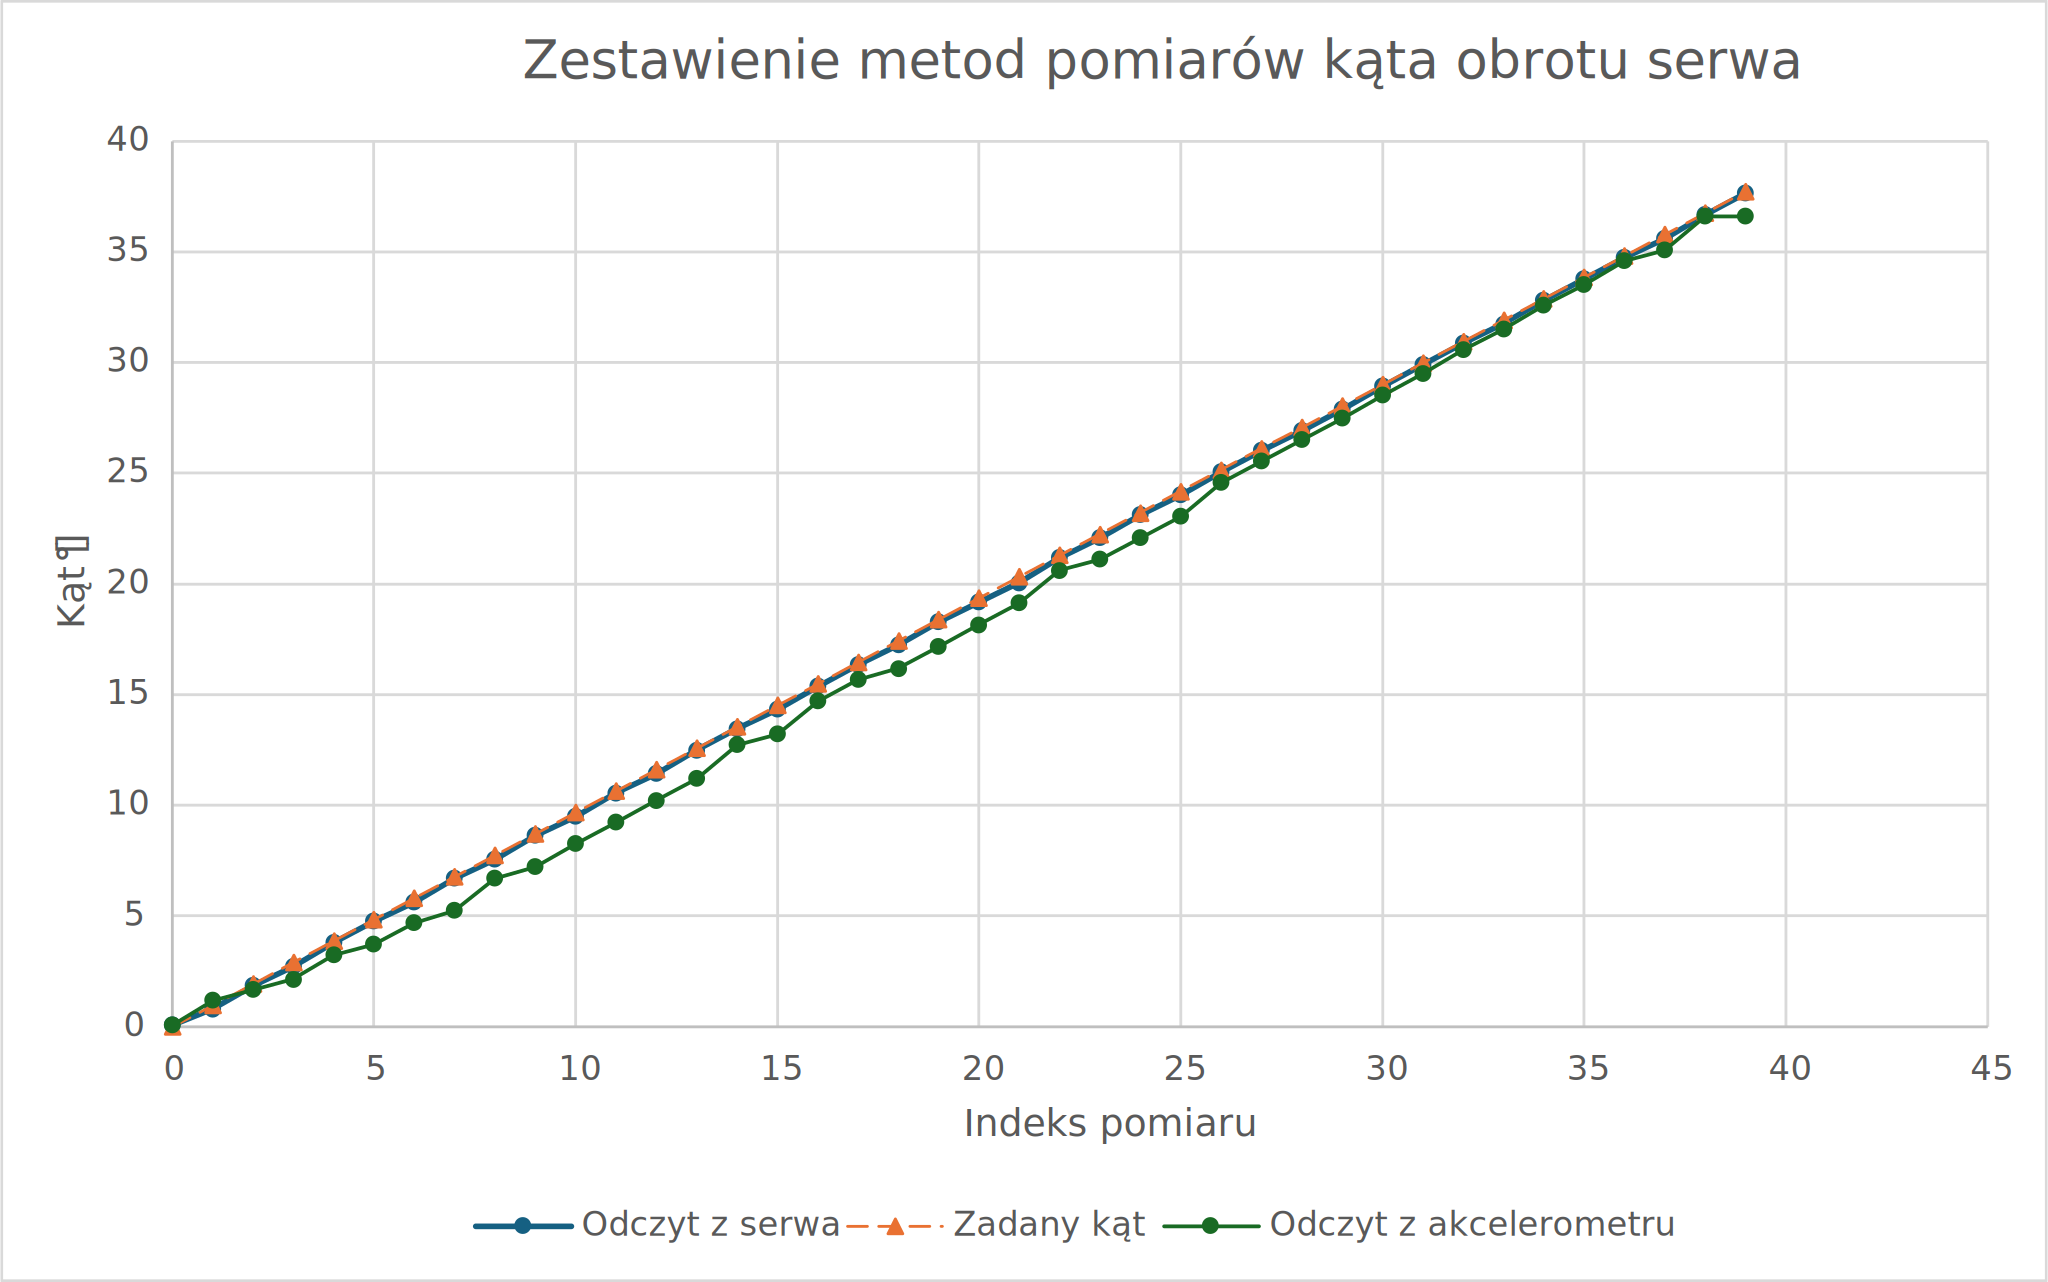
\includegraphics[width=\linewidth]{rysunki/acc/graph.png}
    \caption{Przebieg jednej z serii pomiarowych}
    \label{fig: graph_meas}
\end{figure} 

Wykres \ref{fig: graph_meas} przedstawia jedną ze zmierzonych serii pomiarowych. Uzyskanie wspólnego kąta zerowego dla obu układów zostało osiągnięte przez 'przesunięcie' całej serii pomiarowej akcelerometru o kąt odnotowany dla pomiaru o indeksie zerowym. Wyniki wszystkich serii uśredniono uzyskując następujące dane:

\begin{table}[!ht]
    \centering
    \begin{tabular}{p{3.5cm} | p{3.5cm} | p{3.5cm} | p{3.5cm}}
         Średni uchyb serwa [$\degree$] & Maksymalny uchyb serwa [$\degree$] & Średnia różnica pomiarów [$\degree$] & Maksymalna różnica pomiarów [$\degree$] \\ \hline \hline
         -0,14 & 0,26 & 1,47 & 2,31 \\ 
    \end{tabular}
    \caption{Zestawienie podstawowych danych statystycznych}
    \label{tab: results}
\end{table} 

Na podstawie tabeli \ref{tab: results} widoczne jest, że wysterowanie serwa daje dość satysfakcjonujące rezultaty dając uchyby rzędu 0,1-0,2$\degree$. Niestety jest to uchyb, który trudno wyeliminować ze~względu na~jego niejawny sposób pracy oraz brak możliwości ''ręcznego'' wysterowania urządzenia. Różnica między kątem odczytywanym przez akcelerometr a serwem wynosiła średnio 1,47$\degree$. Jednak w~ogólności widoczne jest, że pomiary są ze sobą zgodne. Prawdopodobną przyczyną takich różnic jest to jak zamocowano akcelerometr. Zarówno kable łączące urządzenie z mikrokontrolerem jak i~niedostatecznie sztywny montaż na orczyku sprawiły, że pomiary były zaburzone. Test należałoby powtórzyć, gdy elementy będą zamontowane w robocie. Wówczas akcelerometr będzie pracował we~właściwych warunkach, dzięki czemu wyniki będą bardziej miarodajne



